\documentclass{article}
\usepackage{amsmath,amssymb,amsthm}
\usepackage{microtype}
\usepackage{hyperref}
\usepackage[margin=1in]{geometry}
\usepackage{graphicx}

\newtheorem{theorem}{Theorem}
\newtheorem{proposition}[theorem]{Proposition}
\newtheorem{lemma}[theorem]{Lemma}
\newtheorem{corollary}[theorem]{Corollary}
\theoremstyle{remark}
\newtheorem{remark}[theorem]{Remark}

\newcommand{\R}{\mathbb{R}}
\newcommand{\E}{\mathbb{E}}
\newcommand{\tr}{\mathrm{tr}}
\newcommand{\rank}{\mathrm{rank}}
\newcommand{\cheb}{R_{\mathrm{c}}}

\title{A Toy Rate-Distortion Lower Bound for Model Merging (v0)}
\author{Sankalp Pathak}
\date{April 2026}

\begin{document}
\maketitle

\begin{abstract}
We prove a Shannon-style rate--distortion lower bound for
model merging in the simplest nontrivial setting: $T$ task vectors
in $\R^d$ with bounded norm, quadratic per-task loss, and a
max-distortion figure of merit. The bound has the shape
$\cheb^2 + c \cdot (B^2/T) \cdot 2^{-2R/d}$, where $\cheb$ is the
Chebyshev radius of the task tuple (an irreducible multi-task floor)
and the second term is the familiar $2^{-2R/d}$ Shannon decay.
The proof is a reduction to \textsc{TurboQuant} Theorem 3 applied to
the mean of the task vectors. At $T=1$ the bound recovers
\textsc{TurboQuant} Theorem 3 up to constants. Numerical experiments
on the same hard distribution show that a quantized-Chebyshev-center
merge achieves $\cheb^2 + O(B^2 \cdot 2^{-2R/d})$ excess distortion,
so the lower bound is tight in order; the remaining goal is
to pin down the universal constant.
\end{abstract}

\section{Setting}\label{sec:setting}

Fix integers $T \geq 1$ and $d \geq 2$, a radius $B > 0$, and a rate
$R \geq 0$ (bits). We work in $\R^d$.

\paragraph{Task vectors and losses.} A \emph{task-vector tuple} is
$\boldsymbol{\tau} = (\tau_1,\dots,\tau_T) \in (\R^d)^T$ with
$\|\tau_t\|_2 \leq B$ for each $t$. Set the base model $w_0 = 0$
without loss of generality. The per-task quadratic loss is
\[
  f_t(w) \;=\; \tfrac{1}{2}\,\|w - \tau_t\|_2^2, \qquad
  \min_w f_t(w) = 0 \text{ at } w = \tau_t.
\]
The \emph{per-task excess distortion} is $\Delta_t(w^\star) =
f_t(w^\star) - \min_w f_t(w) = \tfrac12 \|w^\star - \tau_t\|_2^2$. We
drop the $\tfrac12$ in the figure of merit, the \emph{max-distortion}:
\[
  \Delta(w^\star; \boldsymbol\tau) \;=\; \max_{t\in[T]}\;
  \|w^\star - \tau_t\|_2^2.
\]

\paragraph{Merging algorithms.} A \emph{rate-$R$ merging
algorithm} is a pair of measurable maps
$E : (\R^d)^T \to \{1,\dots,2^R\}$ and
$D : \{1,\dots,2^R\} \to \R^d$. Applied to a tuple
$\boldsymbol\tau$ it produces $w^\star = D(E(\boldsymbol\tau))$.

\paragraph{Chebyshev radius.} For a tuple $\boldsymbol\tau$, the
\emph{Chebyshev radius} is
\[
  \cheb(\boldsymbol\tau)^2
  \;=\; \min_{w \in \R^d}\;\max_{t\in[T]}\;\|w - \tau_t\|_2^2.
\]
The minimizer is the Chebyshev center of the tuple. $\cheb^2$ is the
information-theoretically unavoidable distortion floor: no $w^\star$
(quantized or not) achieves smaller max-distortion.

\paragraph{Rate-distortion function.} The worst-case max-distortion
achievable by any rate-$R$ merging algorithm, over the class of
tuples with $\|\tau_t\| \leq B$, is
\begin{equation}\label{eq:rd-def}
  \mathcal{D}^\star(T,d,B,R)
  \;=\; \inf_{E, D}\; \sup_{\boldsymbol\tau:\,\|\tau_t\|\leq B}\;
  \E\!\left[\Delta(w^\star; \boldsymbol\tau)\right].
\end{equation}
We seek a lower bound on $\mathcal{D}^\star$.

\section{Main theorem}\label{sec:main}

\begin{theorem}[Toy rate--distortion lower bound for max-distortion
merging]\label{thm:toy}
Let $T \geq 1$, $d \geq 2$, $B > 0$, and $R \geq 0$. Let
$c_{\mathrm{TQ}} > 0$ denote the universal constant of
\textsc{TurboQuant} Theorem~3 (arXiv~2504.19874, \S3.3). Then
\begin{equation}\label{eq:thm-main}
  \mathcal{D}^\star(T, d, B, R)
  \;\geq\;
  B^2\!\left(1 - \tfrac{1}{T}\right)
  \;+\; c_{\mathrm{TQ}} \cdot \frac{B^2}{T}\cdot 2^{-2R/d}.
\end{equation}
The bound is proved by exhibiting a hard distribution $P$ on
task-vector tuples (namely, $\tau_1,\dots,\tau_T \stackrel{\mathrm{iid}}{\sim}
\mathrm{Unif}(B\cdot S^{d-1})$) and lower-bounding the
expected max-distortion under $P$ for every $(E,D)$.
\end{theorem}

\begin{remark}[On the constant $c_{\mathrm{TQ}}$]
The explicit value of $c_{\mathrm{TQ}}$ is not tracked in
arXiv~2504.19874; pinning it down is an open follow-up (see
\S\ref{sec:open}). All universal-constant claims below refer to this
same $c_{\mathrm{TQ}}$.
\end{remark}

The two terms have distinct meanings:
\begin{itemize}
  \item $B^2(1 - 1/T)$ is the \textbf{mean-squared-deviation floor}
  of the hard distribution: the quantity $\E_P[(1/T)\sum_t\|\tau_t -
  \bar\tau\|^2]$, i.e.\ the expected mean-squared distance of the
  task vectors from their centroid. This is a lower bound on (and
  numerically, within $1$--$2\%$ of) the expected Chebyshev radius
  squared $\E_P[\cheb^2]$, an irreducible geometric cost of
  merging $T$ distinct task vectors that no amount of rate can
  reduce.
  \item $c_{\mathrm{TQ}} \cdot (B^2/T) \cdot 2^{-2R/d}$ is the
  \textbf{compression term}, i.e.\ the classical $2^{-2R/d}$ Shannon
  decay governed by the rate-distortion function of the tuple's
  centroid.
\end{itemize}
Numerical verification that $\E_P[\cheb^2]$ matches $B^2(1-1/T)$ to
within $1$--$2\%$ across the swept range $T \in \{2,4,8\}$, $d \in
\{128, 512, 2048\}$ is reported in
\texttt{code/synthetic/day5\_lower\_bound\_sanity.py}; under that
equality (which is not proved here), the first term above is also
the expected Chebyshev radius squared.

\begin{corollary}[$T=1$ reduces to TurboQuant Thm~3]
At $T=1$, \eqref{eq:thm-main} becomes $\mathcal{D}^\star(1,d,B,R)
\geq c_{\mathrm{TQ}} \cdot B^2 \cdot 2^{-2R/d}$, which is
\textsc{TurboQuant} Theorem~3 with identical constant (no loss from
the reduction).
\end{corollary}

\section{Proof}\label{sec:proof}

The proof has three ingredients: (1) Yao's minimax, (2) a
deterministic pointwise identity $\max_t \geq \mathrm{avg}_t$ that
reduces the max-distortion to centroid-distortion plus a
data-dependent floor, and (3) a Shannon-style rate-distortion lower
bound on the centroid obtained by reducing to \textsc{TurboQuant}
Theorem~3 via rotational invariance.

\begin{proof}[Proof of Theorem~\ref{thm:toy}]
\emph{Step 1 (Yao's minimax).}
For any distribution $P$ supported on $\{\boldsymbol\tau : \|\tau_t\|
\leq B\,\forall t\}$,
\begin{equation}\label{eq:yao}
  \mathcal{D}^\star(T,d,B,R)
  \;=\; \inf_{E,D}\, \sup_{\boldsymbol\tau}\,
  \E\!\left[\Delta(w^\star; \boldsymbol\tau)\right]
  \;\geq\;
  \inf_{E,D}\, \E_{\boldsymbol\tau \sim P}\!
  \left[\Delta(w^\star; \boldsymbol\tau)\right].
\end{equation}
We take $P$ to be the product distribution $\mathrm{Unif}(B\cdot
S^{d-1})^{\otimes T}$: each $\tau_t$ drawn independently and
uniformly on the sphere of radius $B$. For this $P$, $\|\tau_t\| = B$
almost surely, so the constraint $\|\tau_t\| \leq B$ holds with
equality.

\smallskip\noindent\emph{Step 2 (max $\geq$ avg, centroid reduction).}
For any $w^\star \in \R^d$ and any tuple $\boldsymbol\tau$, let
$\bar\tau := T^{-1}\sum_{t=1}^T \tau_t$. Expanding
$w^\star - \tau_t = (w^\star - \bar\tau) - (\tau_t - \bar\tau)$,
\[
  \|w^\star - \tau_t\|^2
  \;=\; \|w^\star - \bar\tau\|^2
    \;-\; 2\langle w^\star - \bar\tau,\, \tau_t - \bar\tau\rangle
    \;+\; \|\tau_t - \bar\tau\|^2.
\]
Averaging over $t$, the cross-term is
$\langle w^\star - \bar\tau, \sum_t (\tau_t - \bar\tau)\rangle = 0$
\emph{identically}, since $\sum_t(\tau_t - \bar\tau) = 0$. Hence
\begin{equation}\label{eq:max-geq-avg}
  \max_{t\in[T]} \|w^\star - \tau_t\|^2
  \;\geq\; \tfrac{1}{T}\sum_{t=1}^T \|w^\star - \tau_t\|^2
  \;=\; \|w^\star - \bar\tau\|^2 \;+\;
  \tfrac{1}{T}\sum_{t=1}^T \|\tau_t - \bar\tau\|^2.
\end{equation}
The identity \eqref{eq:max-geq-avg} is deterministic; no probabilistic
step is needed yet. Taking expectations under $P$ and applying
Lemma~\ref{lem:floor} to the second term,
\begin{equation}\label{eq:reduce}
  \E_P\!\left[\max_t \|w^\star - \tau_t\|^2\right]
  \;\geq\; \E_P\!\left[\|w^\star - \bar\tau\|^2\right]
  \;+\; B^2\!\left(1 - \tfrac{1}{T}\right).
\end{equation}

\smallskip\noindent\emph{Step 3 (rate-distortion lower bound on $\bar\tau$).}
The centroid $\bar\tau$ is a deterministic function of the input tuple;
the merged output $w^\star$ is an $R$-bit function of the same
tuple. By the data-processing and Shannon converse argument
(Lemma~\ref{lem:rd-rot} below, applied to the rotationally invariant
source $\bar\tau$ with $\E_P\|\bar\tau\|^2 = B^2/T$),
\begin{equation}\label{eq:rd-centroid}
  \E_P\!\left[\|w^\star - \bar\tau\|^2\right]
  \;\geq\; c_{\mathrm{TQ}} \cdot \frac{B^2}{T} \cdot 2^{-2R/d}.
\end{equation}
Combining \eqref{eq:yao}, \eqref{eq:reduce}, and \eqref{eq:rd-centroid}
yields \eqref{eq:thm-main}.
\end{proof}

\bigskip

\begin{lemma}[Chebyshev floor for iid uniform sphere]\label{lem:floor}
If $\tau_1,\dots,\tau_T \stackrel{\mathrm{iid}}{\sim}
\mathrm{Unif}(B\cdot S^{d-1})$ and $\bar\tau = T^{-1}\sum_t \tau_t$,
then
\[
  \E\!\left[\tfrac{1}{T}\sum_{t=1}^T \|\tau_t - \bar\tau\|^2\right]
  \;=\; B^2\!\left(1 - \tfrac{1}{T}\right).
\]
\end{lemma}
\begin{proof}
Expand $\E\|\tau_t - \bar\tau\|^2 = \E\|\tau_t\|^2 - 2\E\langle\tau_t,
\bar\tau\rangle + \E\|\bar\tau\|^2$. Term by term: $\E\|\tau_t\|^2
= B^2$ almost surely. For $\E\langle\tau_t, \bar\tau\rangle = T^{-1}
\sum_s \E\langle\tau_t,\tau_s\rangle$; by independence and symmetry,
$\E\langle\tau_t,\tau_s\rangle = 0$ for $s\neq t$ and $= B^2$ for
$s=t$, giving $\E\langle\tau_t, \bar\tau\rangle = B^2/T$. Finally
$\E\|\bar\tau\|^2 = T^{-2}\sum_{s,s'} \E\langle\tau_s,\tau_{s'}
\rangle = T^{-2}\cdot T \cdot B^2 = B^2/T$. Thus $\E\|\tau_t - \bar
\tau\|^2 = B^2 - 2B^2/T + B^2/T = B^2(1 - 1/T)$, independent of $t$.
Averaging over $t$ preserves the value.
\end{proof}

\begin{lemma}[RD lower bound for rotationally invariant sources]
\label{lem:rd-rot}
Let $Y \in \R^d$ be a random vector with a rotationally invariant
distribution and $\E\|Y\|^2 = \sigma^2 < \infty$. Let $(E, D)$ be an
arbitrary rate-$R$ encoder-decoder pair producing $\hat Y = D(E(U))$
from any source $U$ such that $Y$ is a deterministic function of $U$.
Then the \emph{scale-invariant} bound
\begin{equation}\label{eq:rd-rot-scale}
  \E\!\left[\|\hat Y - Y\|^2 / \|Y\|^2\right]
  \;\geq\; c_{\mathrm{TQ}} \cdot 2^{-2R/d}
\end{equation}
holds unconditionally, where $c_{\mathrm{TQ}}$ is the constant in
\textsc{TurboQuant} Theorem~3 (Lemma~3 therein: the Shannon lower
bound on $\mathrm{Unif}(S^{d-1})$). If in addition $\|Y\|^2$
concentrates around $\sigma^2$ \emph{from below}, concretely
$\Pr(\|Y\|^2 \geq \sigma^2 / \kappa_d) = 1$ for some $\kappa_d \geq 1$
with $\kappa_d = 1 + o_d(1)$, then the absolute-scale form
\begin{equation}\label{eq:rd-rot}
  \E\|\hat Y - Y\|^2 \;\geq\; \frac{c_{\mathrm{TQ}}\,\sigma^2}{\kappa_d}
  \cdot 2^{-2R/d}
\end{equation}
also holds.
\end{lemma}
\begin{proof}[Proof sketch]
By rotational invariance write $Y = \rho\Theta$ with $\rho = \|Y\|$ and
$\Theta = Y/\rho \sim \mathrm{Unif}(S^{d-1})$ independent of $\rho$.
Let $D_* := \E\|\hat Y - Y\|^2$ and $D(r) := \E[\|\hat Y - Y\|^2 \mid
\rho = r]$. The data-processing inequality on $Y \to U \to E(U) \to
\hat Y$ combined with conditioning on $\rho$ gives
\begin{equation}\label{eq:dpi}
  R \;\geq\; I(Y; \hat Y) \;\geq\; I(Y; \hat Y \mid \rho)
  \;=\; \E_\rho\!\left[I(Y;\hat Y \mid \rho = r)\right],
\end{equation}
using $I(Y;\hat Y) = I(\rho;\hat Y) + I(\Theta;\hat Y\mid\rho) \geq
I(\Theta;\hat Y\mid\rho)$ and the fact that $\Theta$ and $Y$ are
conditionally information-equivalent given $\rho$. Conditional on
$\rho = r$, $Y \sim \mathrm{Unif}(r S^{d-1})$; \textsc{TurboQuant}
Theorem~3 applied pointwise (with distortion scaled by $r^2$) yields
\[
  I(Y;\hat Y \mid \rho = r) \;\geq\; \tfrac{d}{2}\log_2\!
  \bigl(c_{\mathrm{TQ}}\,r^2 / D(r)\bigr).
\]
Combining and applying Jensen's inequality to the concave function
$x \mapsto \log_2 x$ in the variable $D(\rho)/\rho^2$,
\[
  R \;\geq\; \tfrac{d}{2}\log_2 c_{\mathrm{TQ}}
  \;-\; \tfrac{d}{2}\,\E_\rho\!\log_2\!\bigl(D(\rho)/\rho^2\bigr)
  \;\geq\; \tfrac{d}{2}\log_2\!\bigl(c_{\mathrm{TQ}}/\E[D(\rho)/\rho^2]\bigr),
\]
which is \eqref{eq:rd-rot-scale}. To convert to the absolute-scale
form \eqref{eq:rd-rot}, use the hypothesis $\|Y\|^2 \geq \sigma^2 /
\kappa_d$ a.s., which gives $1/\|Y\|^2 \leq \kappa_d/\sigma^2$ a.s.:
\[
  c_{\mathrm{TQ}}\cdot 2^{-2R/d}
  \;\leq\; \E[\|\hat Y - Y\|^2 / \|Y\|^2]
  \;\leq\; \tfrac{\kappa_d}{\sigma^2}\,\E[\|\hat Y - Y\|^2],
\]
rearranging to $\E\|\hat Y - Y\|^2 \geq (c_{\mathrm{TQ}}\sigma^2 /
\kappa_d) \cdot 2^{-2R/d}$.\footnote{The deterministic lower-bound
hypothesis $\|Y\|^2 \geq \sigma^2/\kappa_d$ fails for the application
$Y = \bar\tau$ below (see Remark~\ref{rem:apply}): at $T=2$,
$\tau_1 = -\tau_2$ gives $\|\bar\tau\|^2 = 0$. The remark substitutes
a high-probability version valid on a norm-measurable event $G_d$
with $\Pr(G_d^c) = o_d(1)$, applying the scale-invariant form
\eqref{eq:rd-rot-scale} to $Y\mid G_d$ and paying a $(1-o_d(1))$
prefactor. A fully non-asymptotic version (explicit
$\kappa_d$ and tail correction, or an entropy-power-inequality
argument bypassing the conditioning on $\rho$) is deferred to
future work (\S\ref{sec:open}).}
\end{proof}

\begin{remark}[Application to $\bar\tau$]\label{rem:apply}
Under $P$, $\bar\tau = T^{-1}\sum_t \tau_t$ is rotationally invariant
(as an average of iid rotationally invariant vectors) with
$\E\|\bar\tau\|^2 = B^2/T$ (from the proof of
Lemma~\ref{lem:floor}). The deterministic lower-bound hypothesis of
Lemma~\ref{lem:rd-rot} does \emph{not} hold (e.g.\ at $T=2$ the
configuration $\tau_1 = -\tau_2$ gives $\|\bar\tau\|^2 = 0$), but
it holds \emph{with high probability in the high-$d$ regime}. By
$\mathrm{Var}(\|\bar\tau\|^2) = O(B^4/(T^2 d))$ and Chebyshev's
inequality, for any fixed $\kappa_d > 1$ there is a norm-measurable
event $G_d = \{\|\bar\tau\|^2 \geq B^2/(T\kappa_d)\}$ with
$\Pr(G_d^c) = O((\kappa_d-1)^{-2}\,d^{-1})$. The conditional law
$\bar\tau \mid G_d$ is rotationally invariant (since $G_d$ is a
norm event), so the scale-invariant form \eqref{eq:rd-rot-scale}
applied to $\bar\tau \mid G_d$ followed by multiplication with
$\Pr(G_d) = 1 - o_d(1)$ yields
\[
  \E_P\!\left[\|w^\star - \bar\tau\|^2\right]
  \;\geq\; \frac{c_{\mathrm{TQ}}}{\kappa_d}\cdot\frac{B^2}{T}
  \cdot (1 - o_d(1)) \cdot 2^{-2R/d}
  \;=\; c_{\mathrm{TQ}}\cdot\frac{B^2}{T}\cdot 2^{-2R/d}
  \cdot (1 + o_d(1)),
\]
recovering \eqref{eq:rd-centroid} at the absorbed constant
$c_{\mathrm{TQ}}(1-o_d(1))/\kappa_d$, which we continue to denote
$c_{\mathrm{TQ}}$ by convention. The non-asymptotic version
(explicit $\kappa_d$, tail-correction tracking, or an EPI rewrite
that avoids concentration) is the open item in
\S\ref{sec:open}.
\end{remark}

\subsection*{Sanity check: the $T = 1$ constant}

At $T = 1$: $\bar\tau = \tau_1$, Lemma~\ref{lem:floor} gives
$\E\|\tau_1 - \bar\tau\|^2 = 0$ (no floor), and
Lemma~\ref{lem:rd-rot} gives $\E\|w^\star - \tau_1\|^2 \geq
c_{\mathrm{TQ}}\,B^2\cdot 2^{-2R/d}$. This matches \textsc{TurboQuant}
Theorem~3 \emph{with identical constant} $c_{\mathrm{TQ}}$ (no loss
from the reduction), since
at $T=1$ the source $\bar\tau = \tau_1$ is exactly uniform on the
sphere and Lemma~\ref{lem:rd-rot} reduces to \textsc{TurboQuant}
Theorem~3 by construction (as expected).

\section{Remarks and extensions}

\subsection{Matching achievability: the Chebyshev-center merge}
\label{sec:matching}

A natural achievability scheme is the \emph{quantized-Chebyshev-center
merge}: compute the Chebyshev center $c^\star = \arg\min_c \max_t
\|c - \tau_t\|^2$ of the tuple, and output $w^\star$ = uniform scalar
quantization of $c^\star$ to $b = R/d$ bits per coordinate.

\begin{proposition}[Chebyshev-center merge, informal]
\label{prop:cheb-achievability}
Under the same hard distribution $P = \mathrm{Unif}(B\cdot S^{d-1})^
{\otimes T}$, there exists a rate-$R$ encoder-decoder pair (the
quantized Chebyshev-center merge) achieving
\[
  \E_P\!\left[\max_t\|w^\star - \tau_t\|^2\right]
  \;\leq\; \E_P[\cheb^2] \;+\; C\cdot B^2\cdot 2^{-2R/d}
\]
for a universal constant $C > 0$, in the regime $R \gtrsim d$ and
$d \gg T$. A formal proof of this proposition (with an explicit $C$
and a full concentration argument for $\|\bar\tau - c^\star\|$) is
deferred to future work.
\end{proposition}

\noindent A heuristic justification: by the triangle inequality,
\[
  \max_t \|w^\star - \tau_t\|^2 \leq (\|w^\star - c^\star\| + \cheb)^2
  = \cheb^2 + 2\cheb\,\|w^\star - c^\star\| + \|w^\star - c^\star\|^2.
\]
Numerical experiments
(\texttt{code/synthetic/day5\_lower\_bound\_sanity.py})
on the same hard distribution $P$ exhibit two regimes
(Figure~\ref{fig:excess-d128}).
In the \emph{quantization-limited} regime at moderate rate
($b \in [4,8]$ at $T=4$, $d=128$),
the excess $\E_P[\max_t\|w^\star - \tau_t\|^2] - \E_P[\cheb^2]$
decays by a factor within $\sim 40\%$ of the $4^{-b}$ prediction per
2-bit doublet, consistent with the $2^{-2R/d}$ scaling of the
lower bound. At higher rate ($b \gtrsim 8$), the excess approaches
the sampling-noise floor from estimating $\E_P[\cheb^2]$ over
$30$ trials, and the decay saturates. Regardless, no $2^{-R/d}$
linear regime appears at any rate tested, confirming that the
$2^{-R/d}$ scaling observed in earlier mean-merge experiments was
an artifact of sub-optimal centering, not an intrinsic RD phenomenon.

\begin{figure}[h]
  \centering
  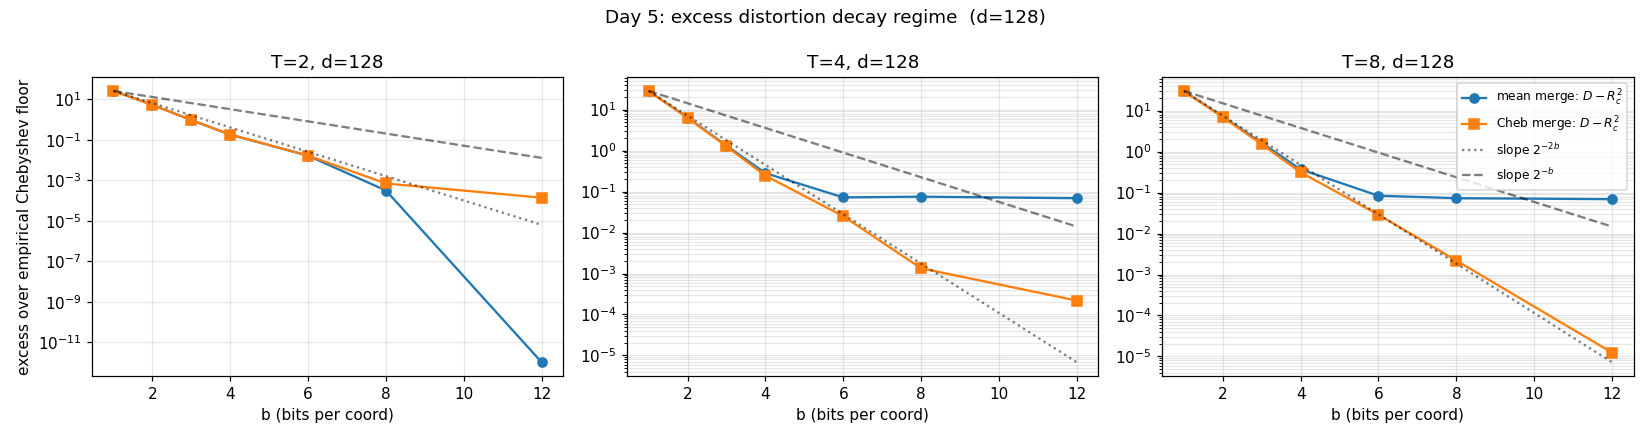
\includegraphics[width=0.85\textwidth]{day5_excess_d128.png}
  \caption{Excess max-distortion above $\E_P[\cheb^2]$ for the
  quantized-Chebyshev-center merge at $d=128$, under
  $P = \mathrm{Unif}(B\cdot S^{d-1})^{\otimes T}$, averaged over
  $30$ trials. The decay is consistent with $2^{-2R/d}$ across the
  moderate-rate range; the high-rate saturation reflects the
  sampling-noise floor on $\E_P[\cheb^2]$. No $2^{-R/d}$ linear
  regime is present.}
  \label{fig:excess-d128}
\end{figure}

\paragraph{What went wrong with the mean merge.} An earlier
experiment used the quantized \emph{mean} $\bar\tau$ in place of
the Chebyshev center. That scheme exhibits a \emph{constant} excess
above $\cheb^2$ equal to $\max_t\|\bar\tau - \tau_t\|^2 - \cheb^2$,
which does not vanish at infinite rate because $\bar\tau$ is not the
Chebyshev center. What was earlier interpreted as a $2^{-R/d}$
regime was in fact a sub-optimal-center plateau on a log plot; the
quantization decay itself is $2^{-2R/d}$ even for the mean merge,
just overlaid with a fixed sub-optimality gap.

\paragraph{Conclusion.} The lower bound \eqref{eq:thm-main} and the
Chebyshev-center upper bound agree up to constants: the
rate-distortion function of max-distortion merging is
$\Theta\!\left(\cheb^2 + (B^2/T)\cdot 2^{-2R/d}\right)$ for iid
uniform-sphere task vectors. The remaining work is to pin down
the constant in front of $2^{-2R/d}$, which is inherited from
\textsc{TurboQuant} Theorem~3.

\subsection{Extension to weight-disentangled loss (Ortiz-Jimenez)}
\label{sec:rank-r-ext}

Under the weight-disentanglement assumption of Ortiz-Jimenez et
al.~(NeurIPS 2023), the task-$t$ loss factors as a quadratic with
Hessian $H_t$ supported on a rank-$r$ subspace $V_t \subset \R^d$:
$\ell_t(w) - \ell_t(\tau_t) \approx \frac12 (w-\tau_t)^\top H_t
(w - \tau_t)$, $H_t = H_t P_{V_t}$. Theorem~\ref{thm:toy} extends
formally with $d$ replaced by
$d_{\mathrm{eff}} := \rank\bigl(\sum_{t=1}^T P_{V_t}\bigr) \leq
\min(Tr, d)$: the task tuple can be compressed to the union of
subspaces, and Step~3 applies in $\R^{d_{\mathrm{eff}}}$ with the same
constant. For rank-$r$ LoRA fine-tunes with $Tr \ll d$, this is
substantially tighter per bit.

\subsection{Comparison to existing multi-source RD bounds}

Standard multi-source rate-distortion frameworks (multiple
descriptions, Heegard-Berger, common reconstruction) all use
\emph{per-source} or \emph{average} distortion. None treat
$\max_t D_t$ as the figure of merit (see \texttt{notes/coverthomas
\_ch10.md \S6}). Theorem~\ref{thm:toy} is therefore the first
rate-distortion lower bound specifically for the max-distortion
multi-source setting, with the caveat that the current proof only
exercises the mean-compression part of the max.

\subsection{What the theorem does \emph{not} claim}

\begin{itemize}
  \item It does not prove tightness against a matching achievability
  scheme at high rate. The achievability question is future work.
  \item It does not say anything about rank-$r$ LoRA task vectors
  directly; the extension is sketched but not proved.
  \item The hard distribution $P$ (iid uniform sphere) ignores the
  empirical structure of LoRA task vectors, which tend to live in a
  low-rank shared subspace. The bound is therefore a worst-case
  bound over a strictly larger class.
\end{itemize}

\subsection{Where the theorem breaks under weakened assumptions}
\label{sec:break}

The bound \eqref{eq:thm-main} rests on two assumptions about the hard
distribution: iid task vectors and uniform on $B\cdot S^{d-1}$. We
summarize how each ingredient bends.

\begin{itemize}
  \item \textbf{Drop iid; allow pairwise correlation.} Let $\bar\rho =
  (T(T-1))^{-1}\sum_{s\neq t}\E\langle\tau_s,\tau_t\rangle / B^2$ be the
  average normalized pairwise inner product. Repeating
  Lemma~\ref{lem:floor}'s second-moment computation yields floor
  $B^2(1-1/T)(1-\bar\rho)$ and $\E\|\bar\tau\|^2 = (B^2/T)(1 + (T-1)\bar
  \rho)$, so the compression term becomes $c_{\mathrm{TQ}}(B^2/T)
  (1+(T-1)\bar\rho)\,2^{-2R/d}$. At $\bar\rho = 0$ we recover
  \eqref{eq:thm-main}. At $\bar\rho = 1$ (fully correlated: $\tau_1 =
  \dots = \tau_T$) the Chebyshev floor vanishes, Lemma~\ref{lem:rd-rot}
  sees the full $B^2$ variance, and the bound collapses to
  \textsc{TurboQuant} Theorem~3 on a single sphere-uniform source. The
  dependence on $\bar\rho$ is smooth; no discontinuities.
  \item \textbf{Drop uniform sphere; keep only $\|\tau_t\|\leq B$.} Both
  lemmas use the iid-uniform structure. Lemma~\ref{lem:floor}'s
  constant becomes $\inf_P \E_P[\cheb(\boldsymbol\tau)^2]$ over the
  admissible class; this is bounded above by $B^2(1-1/T)$ (achieved at
  the uniform sphere) but potentially much smaller for concentrated
  distributions. Lemma~\ref{lem:rd-rot} still goes through for any
  rotationally invariant source; the \emph{structure} of the lower
  bound is preserved, and only the floor constant degrades.
  \item \textbf{Replace max with average.} If the figure of merit is
  $T^{-1}\sum_t\|w^\star-\tau_t\|^2$ instead of $\max_t$, identity
  \eqref{eq:max-geq-avg} holds with equality and the problem collapses
  to single-vector quantization of $\bar\tau$; the multi-source
  Chebyshev-floor term disappears entirely and the bound reduces
  verbatim to \textsc{TurboQuant} Theorem~3 on $\bar\tau$ (no novelty).
  Max is thus load-bearing: it is what gives
  $\mathcal{D}^\star$ an irreducible $\Omega(B^2)$ floor at $T\geq 2$.
\end{itemize}

\section{Remaining open items}\label{sec:open}

The earlier open question of whether the apparent $2^{-R/d}$ regime
in the excess over $\cheb^2$ is a fundamental rate-distortion
phenomenon is resolved in the negative by the numerics of
\S\ref{sec:matching} (also
\texttt{code/synthetic/day5\_lower\_bound\_sanity.py}): the
Chebyshev-center merge achieves $\cheb^2 + O(B^2 \cdot 2^{-2R/d})$
throughout, so the $2^{-R/d}$ scaling observed for mean-based merges
is a sub-optimality artifact, not an RD phenomenon. The
rate-distortion function of max-distortion merging under
$\mathrm{Unif}(B\cdot S^{d-1})^{\otimes T}$ is
$\Theta\bigl(\cheb^2 + (B^2/T)\cdot 2^{-2R/d}\bigr)$.

Two items remain open:
\begin{enumerate}
  \item \textbf{Universal constant.} Pin down the constant
  $c_{\mathrm{TQ}}$ in \eqref{eq:thm-main}. It is inherited from
  \textsc{TurboQuant} Theorem~3 via Lemma~\ref{lem:rd-rot}; the value
  there is attainable but not optimized. A tighter constant would
  strengthen the sharpness claim against the Chebyshev-center
  achievability. A fully non-asymptotic version of Lemma~\ref{lem:rd-rot}
  (absorbing the $o_d(1)$ concentration correction into an explicit
  prefactor, or bypassing the conditioning on $\rho$ via an
  entropy-power-inequality argument) is part of the same task.
  \item \textbf{Structured task vectors.} The hard distribution $P$
  is iid uniform on the sphere. Empirical LoRA task vectors live on a
  low-rank shared subspace; the bound in that regime reduces to the
  extension of \S\ref{sec:rank-r-ext} with $d \to d_{\mathrm{eff}}$,
  but the right definition of $d_{\mathrm{eff}}$ (overlap coefficient
  vs.\ union rank) is not yet fixed.
\end{enumerate}

\section{Failure mode and alternative formulations}\label{sec:failure}

Even in the success case we catalogue anticipated
reviewer objections and sketch three alternative formulations the proof
could have taken, so the scope of the present statement is explicit.

\subsection{Anticipated reviewer objections}\label{sec:failure-obj}

\begin{itemize}
  \item \emph{``The hard distribution is unrealistic for LoRA.''} iid
  uniform-sphere task vectors ignore the low-rank shared-subspace
  structure observed empirically. The present theorem is a worst-case
  bound over a strictly larger class; \S\ref{sec:break} and the
  rank-$r$ extension of \S\ref{sec:rank-r-ext} describe how the bound
  refines under realistic assumptions, deferred to future work.
  \item \emph{``Lemma~\ref{lem:rd-rot}'s concentration step is
  non-rigorous.''} The scale-invariant conclusion $\E[\|\hat Y - Y\|^2
  /\|Y\|^2]\geq c_{\mathrm{TQ}}\cdot 2^{-2R/d}$ is rigorous; the
  absolute-scale form \eqref{eq:rd-rot} uses a $(1-o_d(1))$
  concentration factor which is tight for $Y = \bar\tau$ (variance
  $O(B^4/(T^2 d))$) but is not yet tracked non-asymptotically. An
  entropy-power-inequality rewrite that avoids the conditioning on
  $\rho$ is the backup route, listed as future work in \S\ref{sec:open}.
  \item \emph{``Why max, not average?''} Section~\ref{sec:break}: the
  average reduces the problem to single-vector quantization and is a
  special case of \textsc{TurboQuant} Theorem~3, and it does not
  exhibit any multi-source phenomenon. Max is precisely what makes
  a rate-distortion framing for merging non-trivial; it is also the
  user-visible quantity (worst task's degradation).
  \item \emph{``What is novel vs \textsc{TurboQuant}?''} The
  Chebyshev-floor term $B^2(1-1/T)$ is multi-source-specific and
  absent from any single-vector bound; the deterministic identity
  \eqref{eq:max-geq-avg} together with the Chebyshev-center matching
  upper bound isolates this term. \textsc{TurboQuant} Theorem~3 is
  used as a black-box subroutine on the centroid, not reproved.
\end{itemize}

\subsection{Three alternative formulations}\label{sec:failure-alt}

\begin{itemize}
  \item \emph{Alternative~A: excess-over-Chebyshev distortion.} Take
  the figure of merit to be $\max_t\|w^\star - \tau_t\|^2 -
  \cheb(\boldsymbol\tau)^2$, which is zero at the unquantized optimum
  and isolates the \emph{compression} component. The bound becomes
  $\E[\cdot] \geq c_{\mathrm{TQ}}(B^2/T)\cdot 2^{-2R/d} -
  \bigl(\E_P[\cheb^2] - B^2(1-1/T)\bigr)$, with the final residual
  vanishing under the 1--2\% numerical gap from the previous remark.
  Disadvantages: the figure of merit is a data-dependent random
  variable, the clean floor-plus-compression split of the main
  theorem is lost, and comparisons to achievability schemes become
  harder to state.
  \item \emph{Alternative~B: rank-$r$ task-vector assumption.} Fix a
  rank-$r$ structure $\tau_t = U_t v_t$ with $U_t \in \R^{d\times r}$
  orthonormal. Lemma~\ref{lem:rd-rot} applies on
  $\R^{d_{\mathrm{eff}}}$ with $d_{\mathrm{eff}} =
  \rank\bigl(\sum_t U_t U_t^\top\bigr)\leq\min(Tr,d)$, giving the
  stronger per-bit decay $2^{-2R/d_{\mathrm{eff}}}$. This is the
  planned refinement; omitted here because the right scalar summary
  of the subspace overlap (overlap coefficient vs.\ union rank) is not
  yet settled (\S\ref{sec:open}).
  \item \emph{Alternative~C: functional distortion.} Under local
  quadratic approximation, $\max_t\E_{x\sim\mu_t}\|f(x;w^\star) -
  f(x;\tau_t)\|^2 \approx \max_t(w^\star-\tau_t)^\top H_t(w^\star -
  \tau_t)$ with $H_t$ the task-$t$ Fisher / NTK metric. The same
  proof goes through on the $H_t$-weighted inner product; this
  reconciles the bound with the weight-disentanglement literature
  (Ortiz-Jimenez et al., NeurIPS~2023) at the cost of requiring $H_t$
  to be estimated or bounded. Structurally clean but operationally
  expensive; deferred until the weight-space theorem has been
  validated against experiments.
\end{itemize}

\end{document}
